\documentclass[../main.tex]{subfiles}

\begin{document}

We can use "The World \& The Machine" model by M. Jackson and P. Zave to make an initial domain analysis. This allows us to understand which are the entities and the phenomena the machine cannot directly observe ("The World"), which are the ones the external world cannot directly see ("The Machine"), and the ones that are shared, i.e. the mean of interaction between the two.

\begin{figure}[h!]
	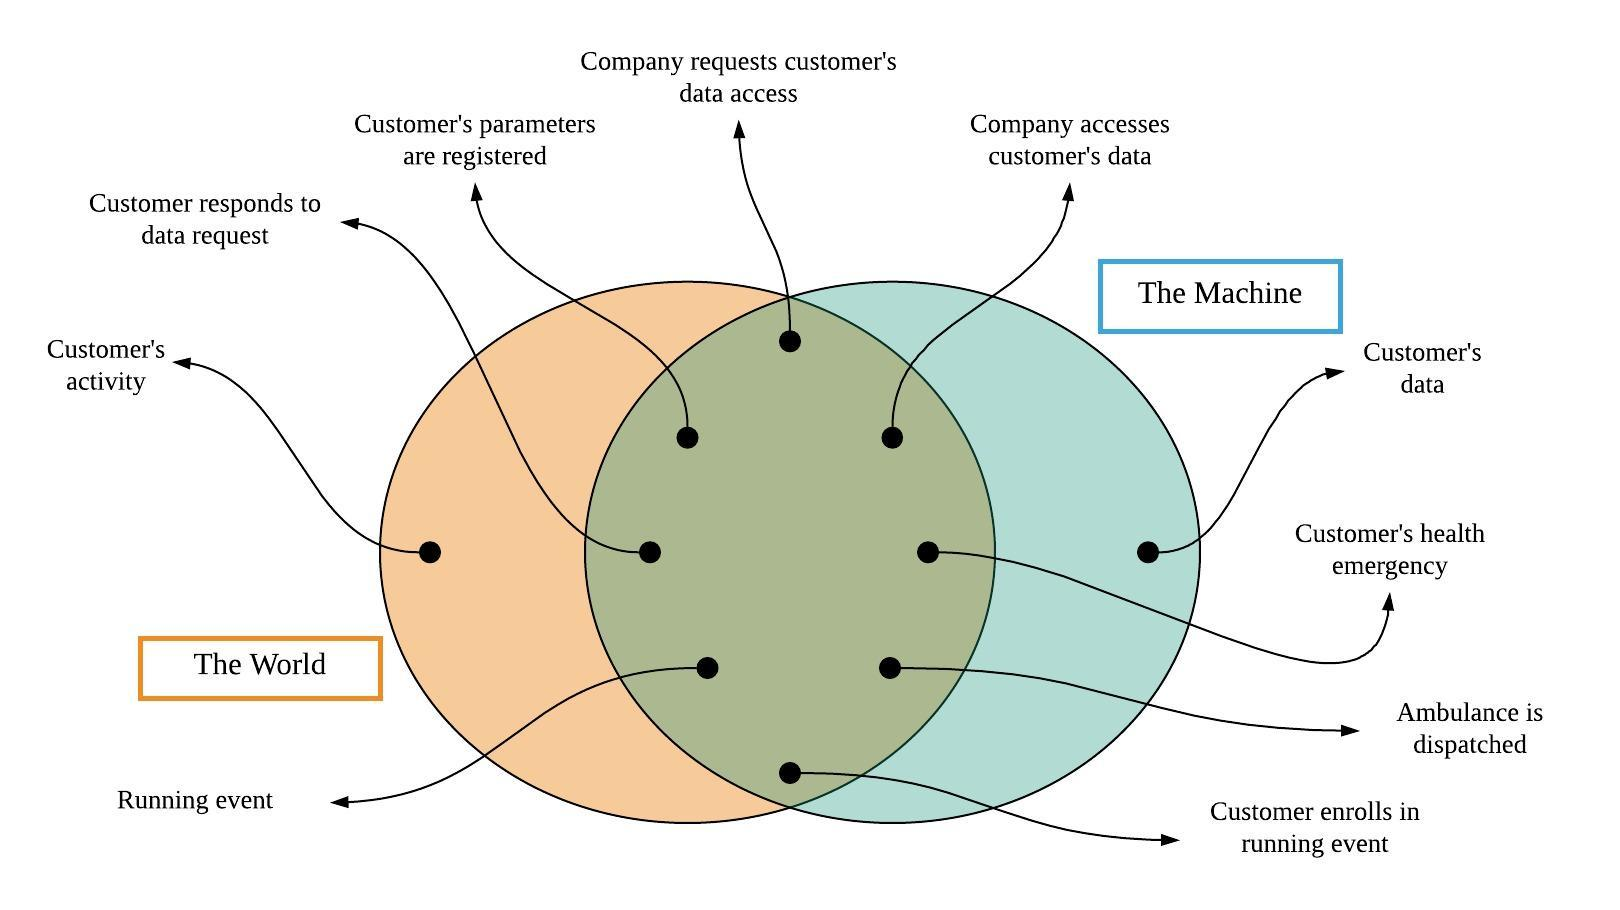
\includegraphics[width=\linewidth]{rasd_worldmachine.jpg}
	\caption{Program analysis as per "The World \& The Machine" model}
	\label{fig:rasd_worldmachine}
\end{figure}

\subsection{Product perspective}

\subsubsection{Class diagrams}

Following there are the class diagrams that give an overall description of our main three services through the use of a conceptual model. Only the relevant parts of the system are present in every one of them for the sake of clarity, but it is to be considered as a single model.
\newpage
\thispagestyle{empty} % yo hide page numbers
\begin{figure}[H]
	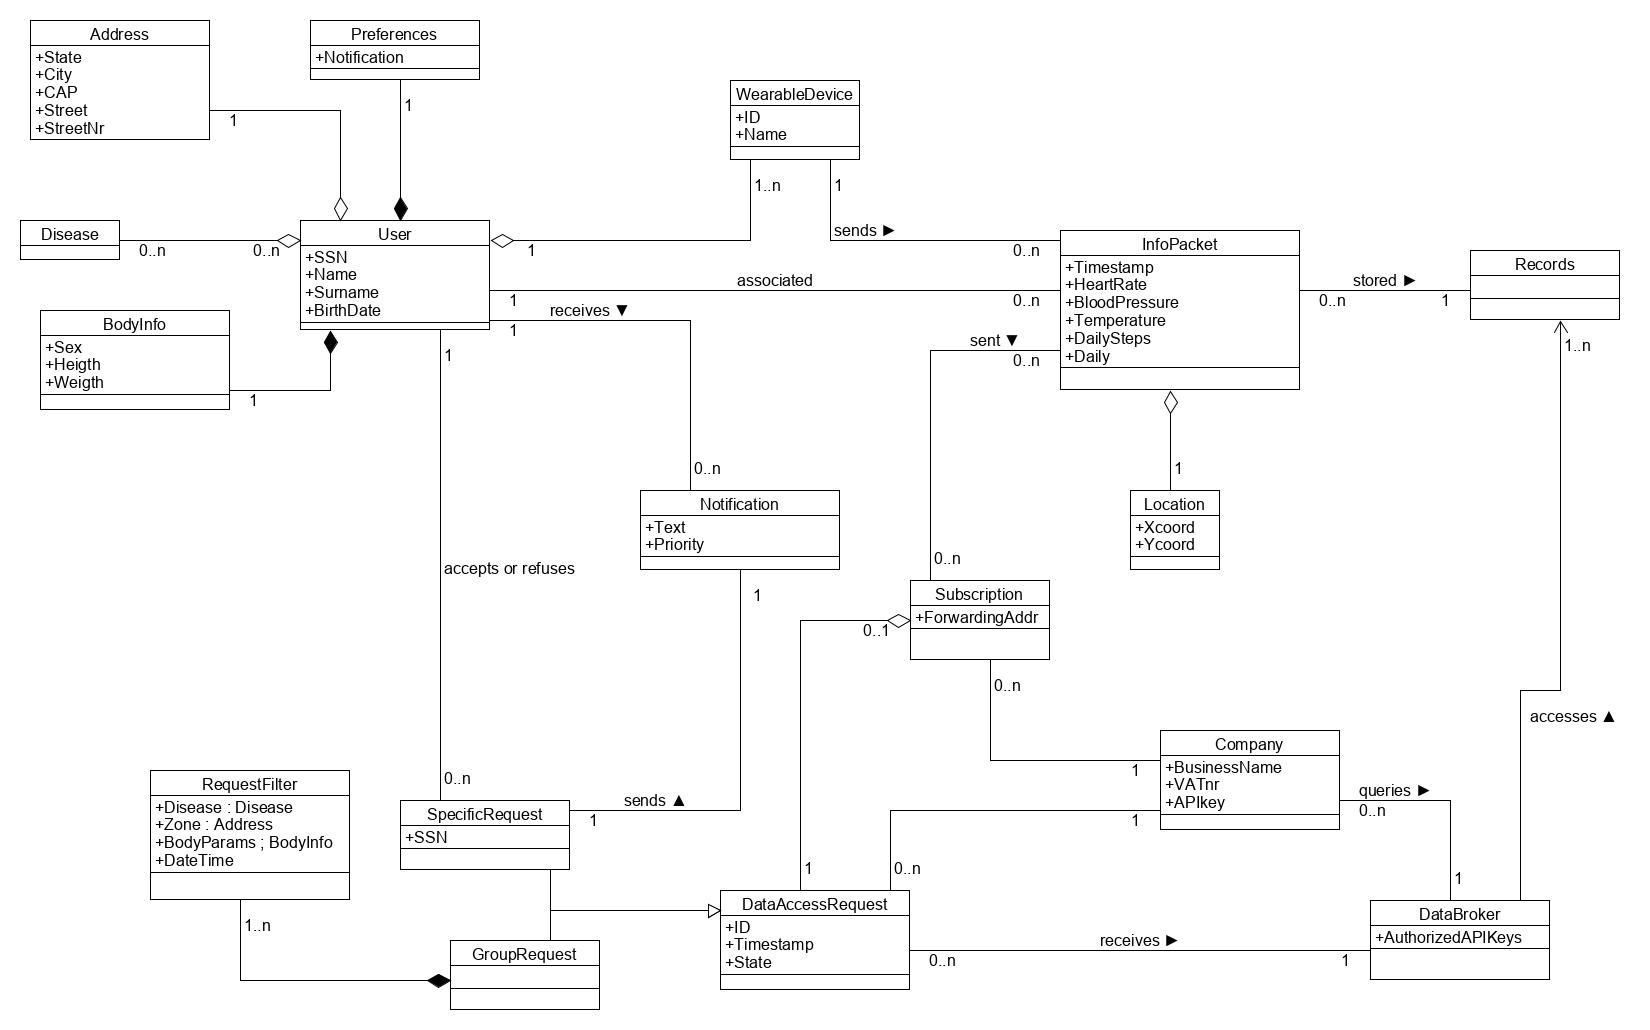
\includegraphics[width=\paperwidth, angle=90]{rasd_classdiag_d4h.jpg}
	\caption{Class diagram for the Data4Help service}
	\label{fig:classdiag_d4h}
\end{figure}
\newpage
\thispagestyle{empty}
\begin{figure}[H]
	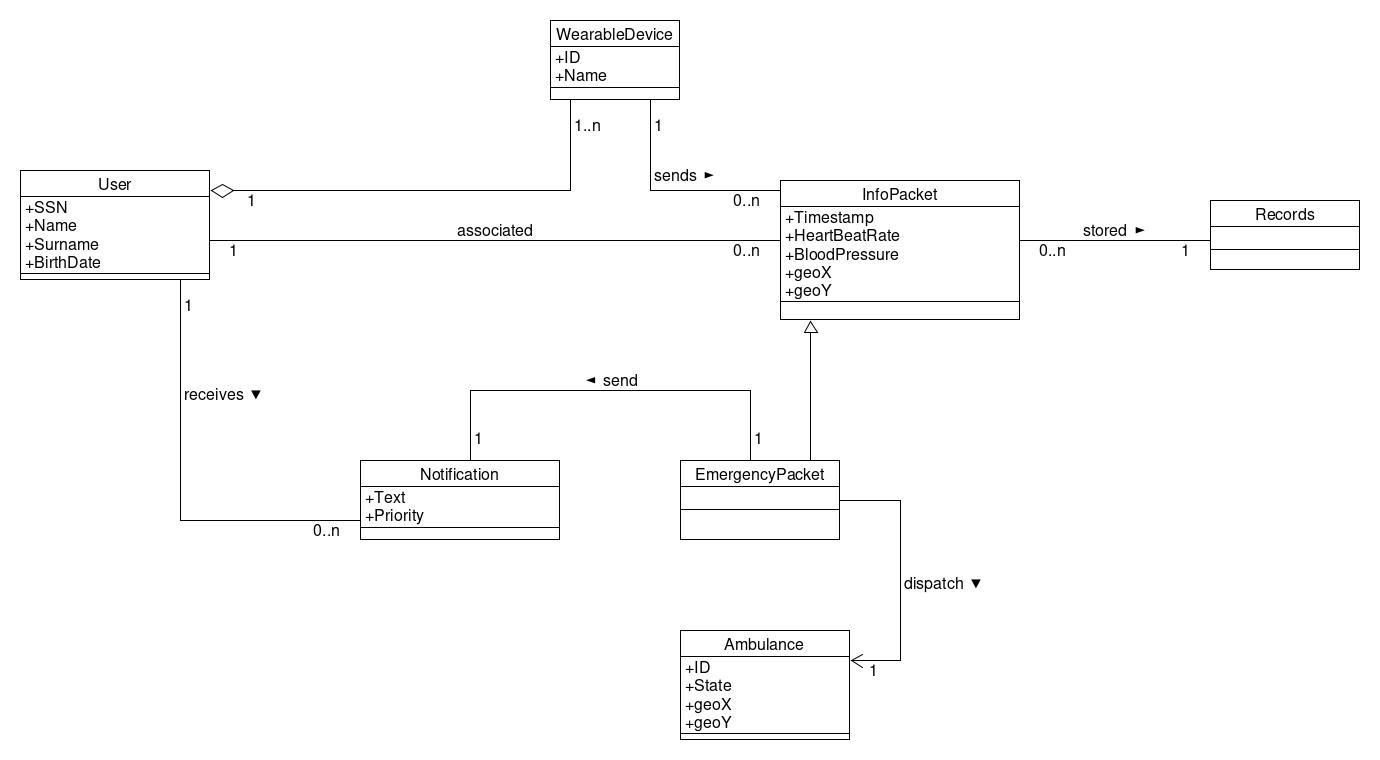
\includegraphics[width=\paperwidth, angle=90]{rasd_classdiag_sos.jpg}
	\caption{Class diagram for the AutomatedSOS service}
	\label{fig:classdiag_sos}
\end{figure}
\newpage
\thispagestyle{empty}
\begin{figure}[H]
	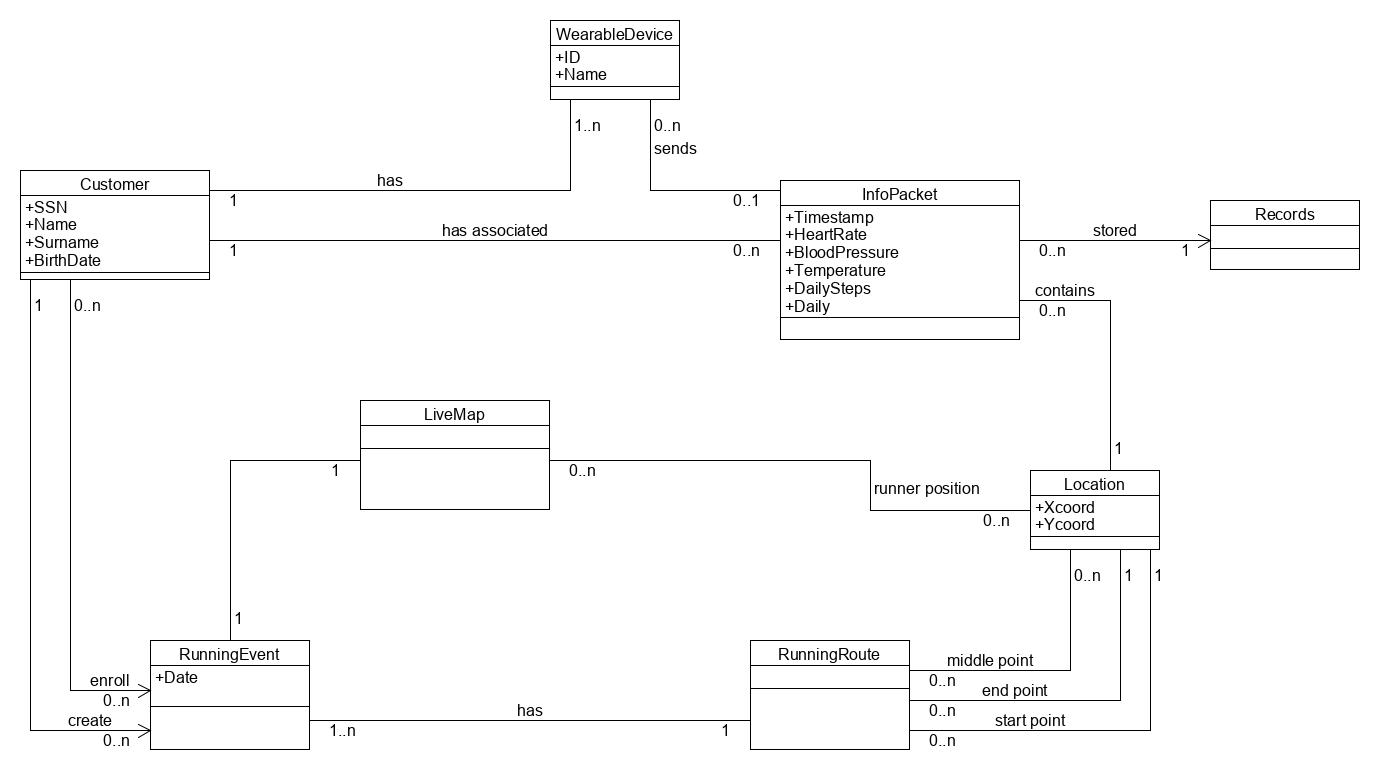
\includegraphics[width=\paperwidth, angle=90]{rasd_classdiag_t4r.jpg}
	\caption{Class diagram for the Track4Run service}
	\label{fig:classdiag_t4r}
\end{figure}
\newpage

\subsubsection{State machine diagrams}

Through the use of the state machine UML model, we desribe the evolution of the states for the main components of the system.

\begin{figure}[H]
	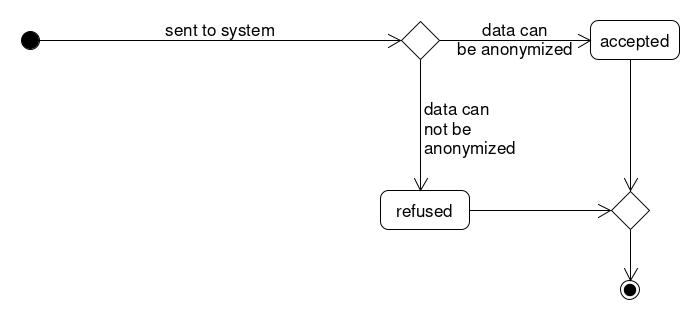
\includegraphics[width=\linewidth]{rasd_statemachine_grpreq.jpg}
	\caption{Statechart of a request for a group of cutsomers data}
	\label{fig:statemachine_grpreq}
\end{figure}

\begin{figure}[H]
	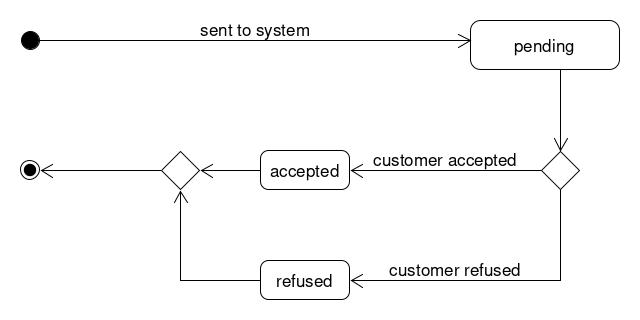
\includegraphics[width=\linewidth]{rasd_statemachine_specreq.jpg}
	\caption{Statechart of a request for a single cutsomer's data}
	\label{fig:statemachine_specreq}
\end{figure}

\begin{figure}[H]
	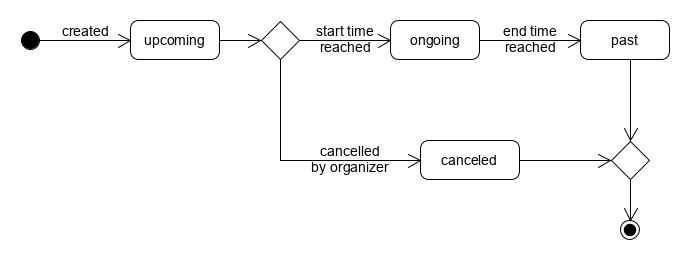
\includegraphics[width=\linewidth]{rasd_statemachine_runevent.jpg}
	\caption{Statechart of a running event}
	\label{fig:statemachine_runevent}
\end{figure}

\subsection{Product functions}

Following are the requirements our system has to satisfy in order to provide the main functionalities, each associated with its proper goal.

\begin{minipage}{\textwidth}
\vspace{4mm}
{\bf Data4Help}
\begin{description}
	\item [G1]  Third parties shall be able to make requests for accessing single customer data.
	\begin{description}
		\item [R1] The system must forward any request from a company to single customer's data to the corresponding user.
	\end{description}

	\item [G2]  Third parties shall be able to make requests for accessing aggregate anonymous data specifiying filters.
	\begin{description}
		\item [R2] The system must reject any request for data regarding a group of customers when it cannot guarantee the anonimity of its components.
	\end{description}

	\item [G3]  Third parties shall be able to access stored data, for which a request has been approved.
	\begin{description}
		\item [R3] The system must periodically collect and store customer's data.
	\end{description}

	\item [G4]  Third parties shall be able to subscribe to new data, for which a request has been approved.
	\begin{description}
		\item [R4] The system must periodically update the accessible data with the newly collected one.
	\end{description}

	\item [G5]  Users shall be able to accept or refuse requests for their data from third parties.
	\begin{description}
		\item [R5] The system must notify the user of the request and permit him to accept or refuse it.
		\item [R6] The system must update the request status with the answer provided by the user.
	\end{description}

	\item [G6]  Access to customers data from a third party, for which a request does not exist, or has been rejected, shall be denied.
	\begin{description}
		\item [R7] The system must be able to identify which data can be accessed for each third party company.
	\end{description}
\end{description}
\end{minipage}
\vspace{8mm}


\begin{minipage}{\textwidth}
{\bf AutomatedSOS}
\begin{description}
	\item [G7]  From the time a customer's parameters indicate a health emergency status, an ambulance shall be dispatched to his location in less than 5 seconds.
	\begin{description}
		\item [R8] The system must continuously check the data read from customers subscribed to AutomatedSOS.
		\item [R9] In case the data indicate an emergency for a customer, the system must dispatch the closest ambulance to his location.
	\end{description}

	\item [G8]  When an ambulance is dispatched, the customer shall be notified of its arrival.
	\begin{description}
		\item [R10] After an ambulance is dispatched, the system must notify the customer of its arrival.
	\end{description}
\end{description}
\end{minipage}
\vspace{8mm}


\begin{minipage}{\textwidth}
{\bf Track4Run}
\begin{description}
	\item [G9]  Organizers shall be able to create a new running event.
	\begin{description}
		\item [R11] The system must allow users to define the route, the date and the time of the event.
		\item [R12] Two events can't overlap in the same place, date and time.
		%\item [R13] When an event is deleted the participants will be notified.
	\end{description}

	\item [G10]  Runners shall be able to view and enroll in available runs.
	\begin{description}
		\item [R13] The system must show open events to the users.
		\item [R14] The system must allow users to sort and filter events by date and location.
	\end{description}

	\item [G11] Spectators shall be able to see the position of participants on the map during a run.
	\begin{description}
		\item [R15] The system must collect and provide in real time the position of participants on a map.
	\end{description}
\end{description}
\end{minipage}
\vspace{8mm}

\subsection{User characteristics}
The service is addressed to two type of costumers:
\begin{itemize}
	\item Third party companies that need data for their own purpose and they can't do it by theirselves or they don't want to do it.
	\item People that want help in case of emergency with autaomatically calling an ambulance and people that want to organize, paricipate or being spectators of run events.
\end{itemize}

\subsection{Assumptions, dependencies, constrains}

{\bf Domain assumptions}

\begin{description}

	\item [D1] Third parties are able to identify specific customers by SSN or FC.
	\item [D2] A group is considered anonymous if is composed by more than 1000 people.
	\item [D3]  A sent request is always received by the targeted user
	\item [D4] Health emergency status occurs when a AutomatedSOS customer parameters falls below or exceeds healthy boundaries.
	\item [D5] AutomatedSOS customers are always connected to GSM or internet.
	\item [D6] An ambulance is always available for dispatching and can reach the customer position.
	\item [D7] Organizers choose a valid path for the event.
	\item [D8] The event is legally autorized by authorities.

\end{description}

\end{document}
